The data we will be using to generate our results comes from three sources, AQS sites, IMPROVE sites, and evaluations of the Downscaler model.  The data we looked at was data collected in Quarter 1.  That is, the data we are considering was collected in January, February, and March.  The methodology we will develop below can be extended to any quarter of the year.  Below, we will discuss how the data source is collected, why the data source is beneficial, and the limitations we have using the data.  We will begin with the data collected at the AQS sites.  

The AQS data was collected at AQS sites.  These sites have AQS machines on the ground to collect concentrations of pollutants (specifically PM-25, the pollutant we are interested in).  We will henceforth refer to this data as "AQS data" or "the ground truth."  While we do have actual readings of the concentration of PM-25, this data is usually only collected near large cities.  The reason for this is that there is legislation that requires cities of certain populations to purchase a machine and then use it to collect readings ofs pollution in the air.  Additionally, the data is not collected every day.  For example, there are locations that collect data every 6 six days.  As a result, it is difficult to get a consistent amount of reliable data from these machines.  Note also that we are not considering the effects of noise in data collection (i.e. no measurement noise in our data collection).

Our second source of data comes from IMPROVE sites.  These sites are again measuring the concentration of the pollutant PM-25 in the air.  Unlike the AQS sites, these sites are located in areas in which there is not a high concentration of the pollutant.  For instance, the IMPROVE sites can be located in a National Park or other rural areas.

Our last piece of data we will be using is from a model called Downscaler (DS).  This model works on a grid, the continental United States divided into 12km by 12km pieces.  It essentially uses a "fancy" linear regression to incorporate the data gathered from the AQS sites and another source of information that indicates the type of environment the grid block is located at.  The output of Downscaler is a mean and standard error for each grid point.  Because the Downscaler is an evaluation of a model, we can choose the area in which we run the model.  This is the source of our problem.  Normally, the Downscaler is ran on a national scale.  That is, it incorporates all of the data from the AQS sites located in the continental United States.  The potential problem with this, is that if the location we are trying to extrapolate is in the NW, the model considers the readings of the AQS machines in the SE.  The hypothesis is that while there is some correlation between the regions in close proximity to each other, overall, the concentrations of PM-25 on one side of the country do not have an effect on the readings on the other side of the country.  The proposed solution is to run the Downscaler on a regional scale with overlapping areas in-between the regions.  That way, a specific grid point only includes information that is "relevant" to the region that it is in.  We include an overlap region because it is assumed that the grid points on the edge of the boundary will be impacted by the near-by grid points in the adjacent region.  Two questions arise from this proposed solution: what regions should be used? and how do we deal with the overlapping region?.

We will address the first question by splitting the continental United States by the NOAA climate zones.  This means that we will have nine regions that we are running the Downscaler on.  The nine regions are Northwest (NW), North Rockies (NR), Upper Midwest (UM), Ohio Valley (OV), Northeast (NE), Southeast (SE), South (S), Southwest (SW), and West (W).  Recall that we are considering these zones plus some overlap into the adjacent regions.  Figure \ref{US} shows the continental US broken up into the NOAA Climate Zones.

% % % %WE STILL NEED TO CITE THIS!!!!!!!!!!!!!!!!!!!
\begin{figure} %[!h]
\begin{center}
  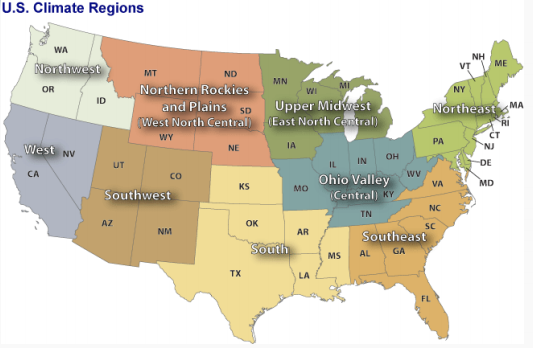
\includegraphics[width=3.9in]{ContUS.png}
\end{center}
\vspace{-0.15truein}
\caption{NOAA Climate Zones.}
\label{US}
\hspace{1.70in}
\vspace{-0.15truein}
\end{figure}

The second question is the reason for which we are writing this paper.  Because we are running the Downscaler for each region plus some overlap, The overlap area will have two (or more) DS values for which the Downscaler model provides an evaluation at each gridpoint.  This paper seeks to provide a methodology for this overlap region.  An example of the overlap region is provided in Figure \ref{overlap}.  Notice that the boxes represented by the dashed lines are the NOAA Climate Zones, i.e. they are a collection of states defined by NOAA in which the states have similar climates.  The two regions that we ran Downscaler on are represented by the solid lines.  By running the Downscaler twice, in the overlap region (which includes the NOAA Climate Zone boundary) we have an evaluation of Downscaler at each grid point.  As a result, we need to find a way to combine the two evaluations into one that makes sense for the grid point.

\begin{figure} %[!h]
\begin{center}
  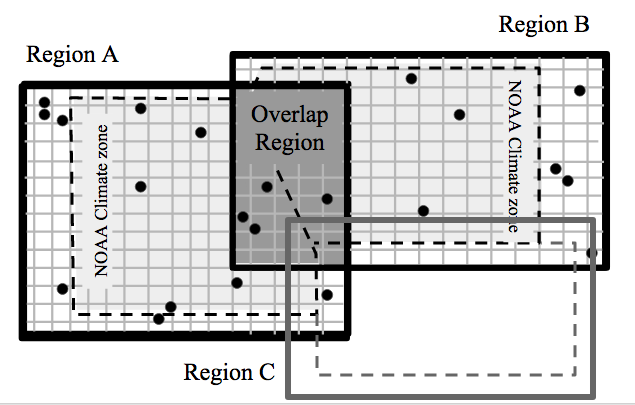
\includegraphics[width=5.9in]{overlap.png}
\end{center}
\vspace{-0.15truein}
\caption{Overlap region on NOAA Climate Zones.}
\label{overlap}
\hspace{1.70in}
\vspace{-0.15truein}
\end{figure}